\begin{center}
\textbf{Лабораторная работа №1}
\\
\textbf{Тема:} Работа с системами контроля версий
\\
\end{center}
\textbf{Задание:} 
\begin{enumerate}
\item Зарегистрироваться на https://github.com/
\item Склонировать репозиторий шаблонов tex https://github.com/egorpugin/tex;
\item Подготовить шаблон отчёта для лабораторных работ в LaTeX;
\item Загрузить шаблон в репозиторий tex;
\item Создать новый репозиторий для лабораторных работ на гитхабе;
\item Оформить отчёт и загрузить его в репозиторий для ЛР;
\\
\end{enumerate}
\begin{figure}[h]
\centering
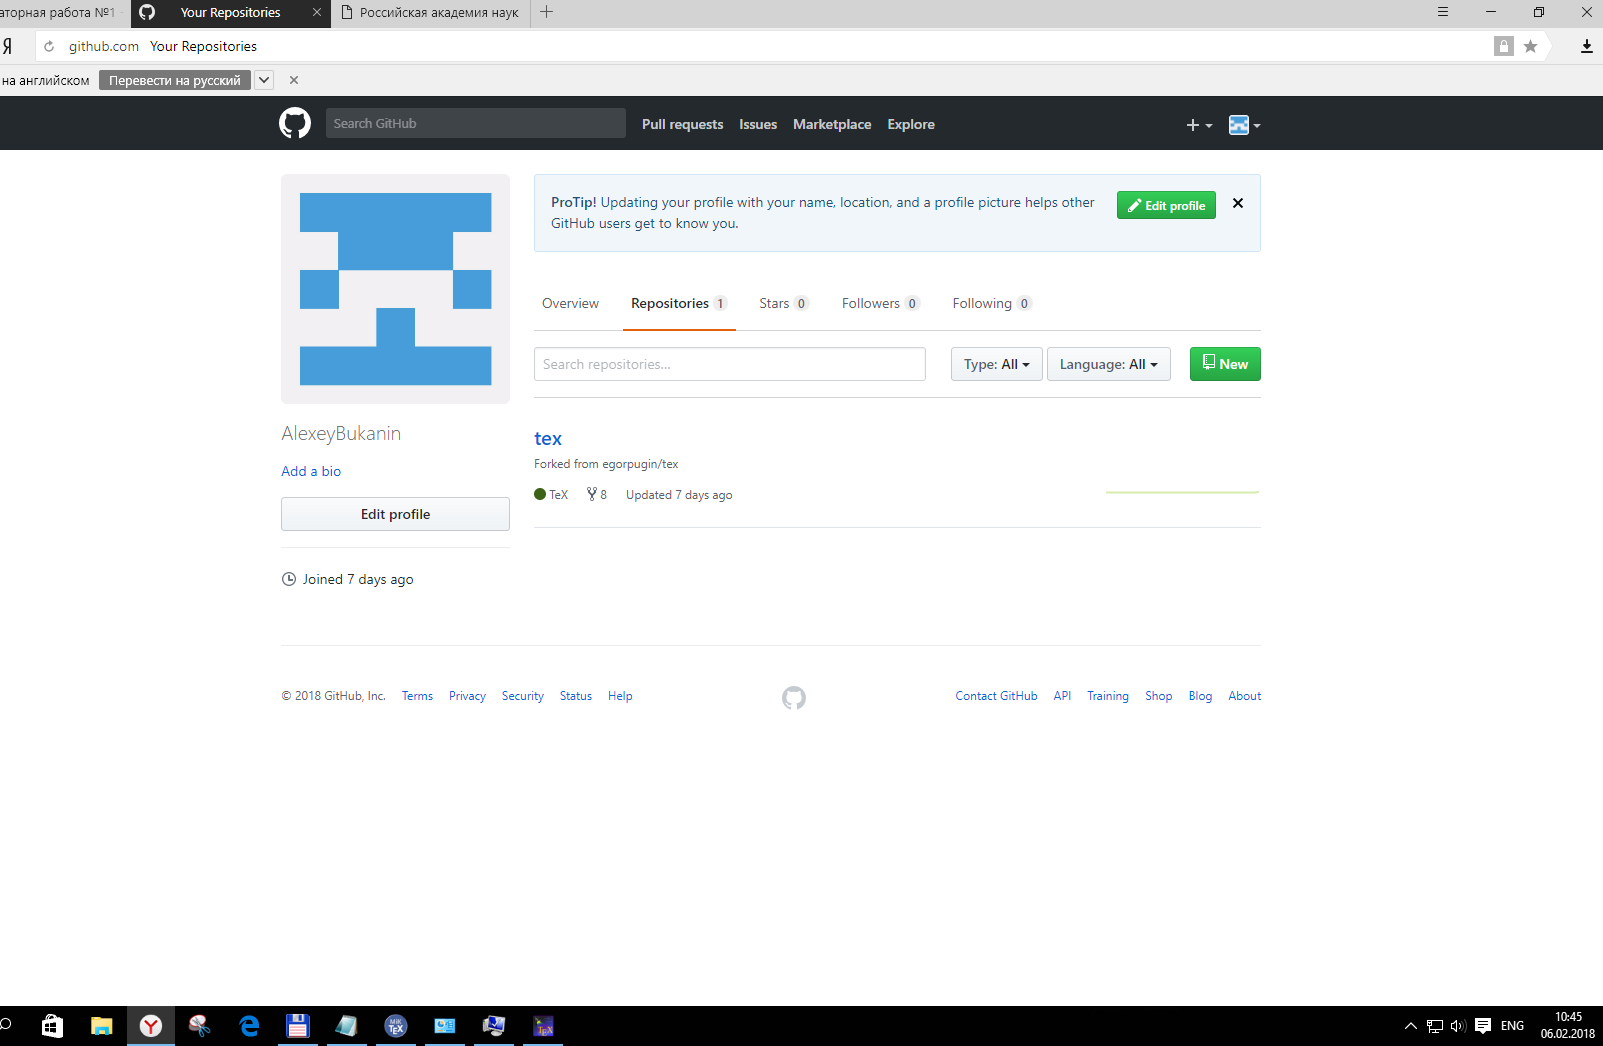
\includegraphics[scale=0.4]{repoz}
\caption{Сайт github.com}
\label{fig:repoz}
\end{figure}

\newpage
\begin{enumerate}
\item Создали репозиторий
\item Добавили файл
\item Зафиксировали изменения
\item Отправили на github

\end{enumerate}

\begin{figure}[h]
\centering
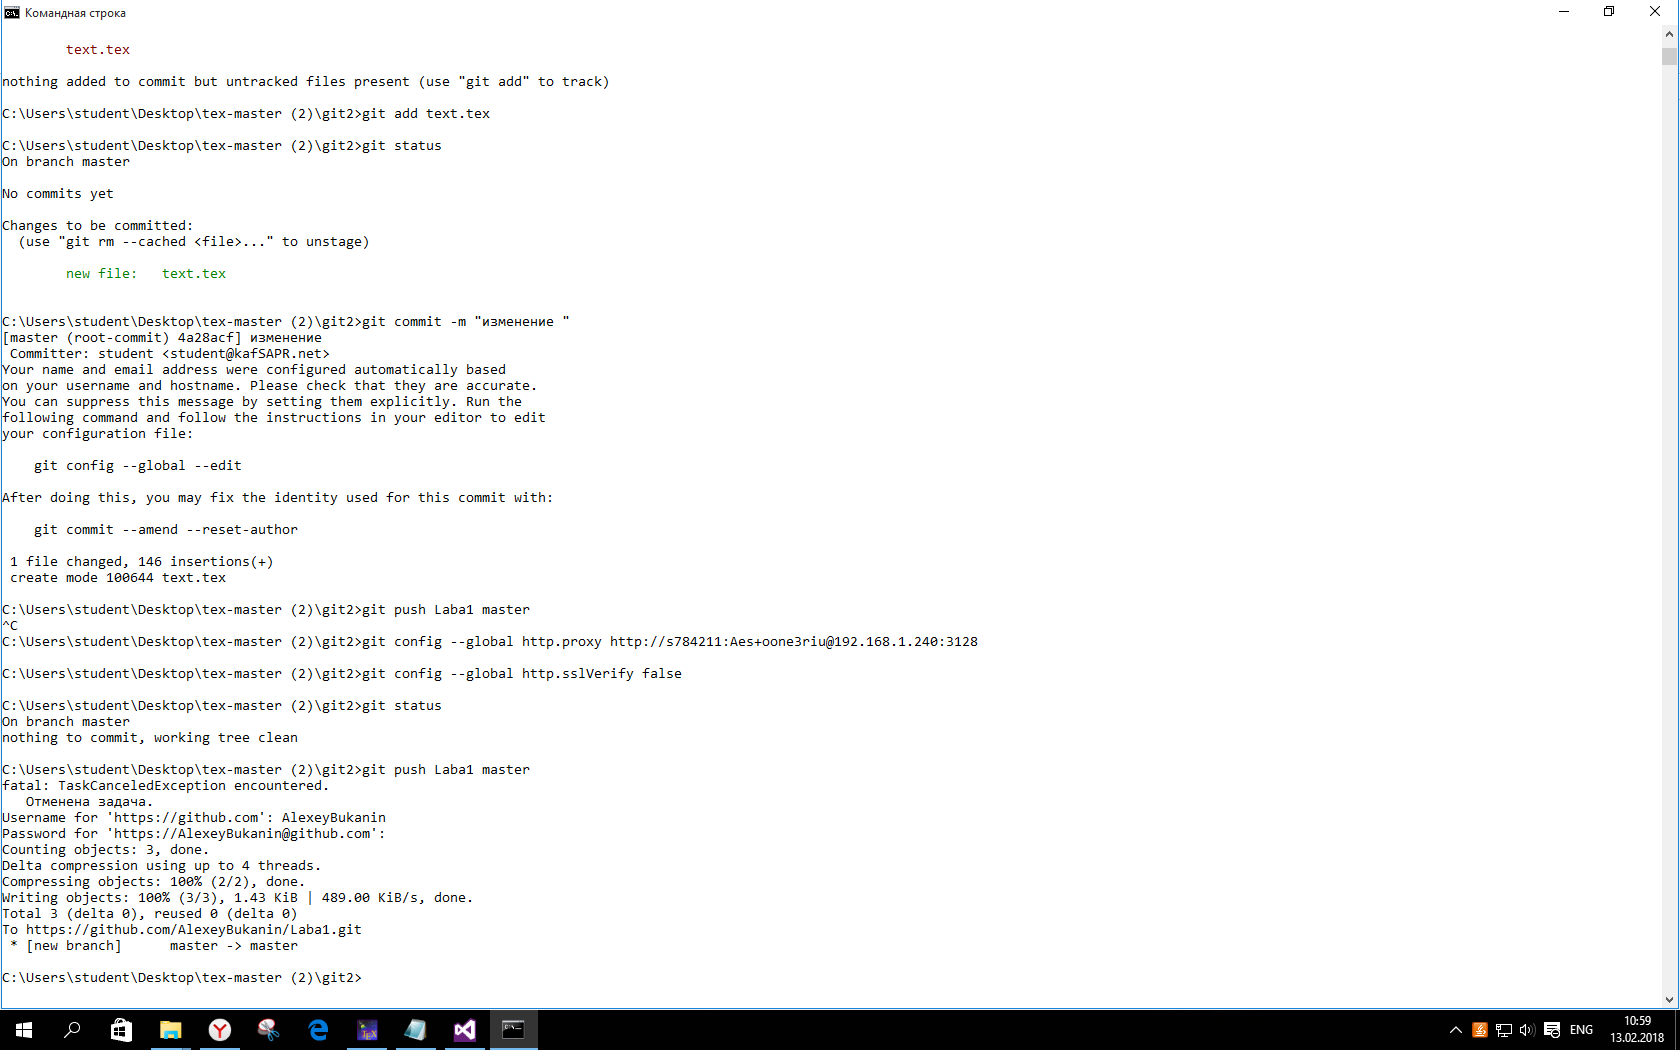
\includegraphics[scale=0.4]{com}
\caption{Используемые команды}
\label{fig:com}
\end{figure}

\newpage

\begin{figure}[h]
\centering
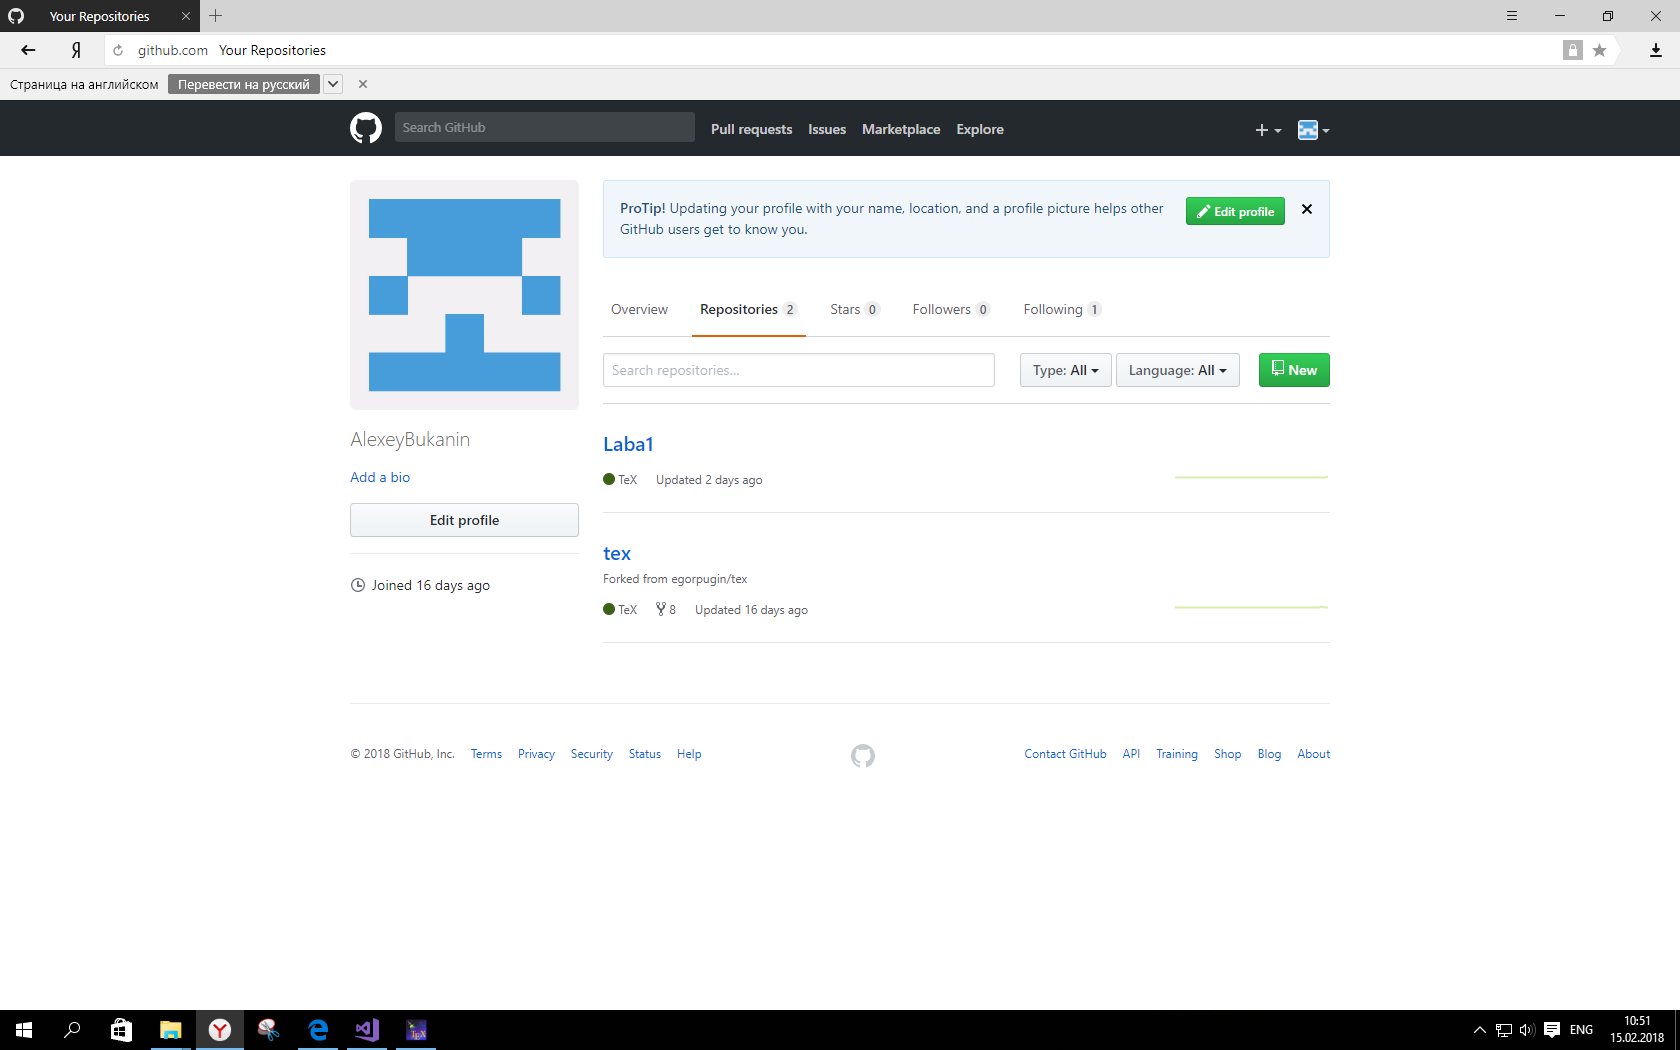
\includegraphics[scale=0.4]{Безымянный}
\caption{Результат}
\label{fig:Безымянный}
\end{figure}



\textbf{Вывод:} Я научился работать с gitom



